
%(BEGIN_QUESTION)
% Copyright 2012, Tony R. Kuphaldt, released under the Creative Commons Attribution License (v 1.0)
% This means you may do almost anything with this work of mine, so long as you give me proper credit

Anta at en radiosender leverer 0.75 watt effekt inn i den ene enden av en tvillingleder-kabel, med antennen koblet i den andre enden. Kabelen er 20 fot lang og har et effekttap på $-0.033$ dB/fot. Beregn effekten mottatt av antennen, både i watt og i dBm.

\vskip 10pt

$P_{antenna}$ = \underbar{\hskip 50pt} watt

\vskip 10pt

$P_{antenna}$ = \underbar{\hskip 50pt} dBm

\vskip 20pt \vbox{\hrule \hbox{\strut \vrule{} {\bf Forslag til sokratisk diskusjon} \vrule} \hrule}

\begin{itemize}
\item{} En sterkt anbefalt teknikk for tekstoppgaver er å {\it tegne en skisse} av problemet og merke elementene i skissen med gitt informasjon. Gjør dette, og sammenlign skissen din med medstudentenes. Hvordan hjelper dette konkret i problemløsningen?
\item{} Løs denne oppgaven på mer enn én måte, og forklar hvordan de ulike løsningene fungerer.
\item{} Forklar hva ``dBm'' faktisk {\it betyr}. Enkle tall-eksempler kan være nyttige:
\begin{itemize}

\item{} Hvor mye effekt er +3 dBm?
\item{} Hvor mye effekt er $-3$ dBm?
\item{} Hvor mye effekt er +10 dBm?
\item{} Hvor mye effekt er $-10$ dBm?
\end{itemize}
\end{itemize}

\underbar{file i01204}
%(END_QUESTION)





%(BEGIN_ANSWER)

$P_{antenna}$ = \underbar{\bf 0.644} watt

\vskip 10pt

$P_{antenna}$ = \underbar{\bf 28.09} dBm

%(END_ANSWER)





%(BEGIN_NOTES)

Å tegne en skisse av problemet anbefales sterkt som problemløsningsteknikk:

$$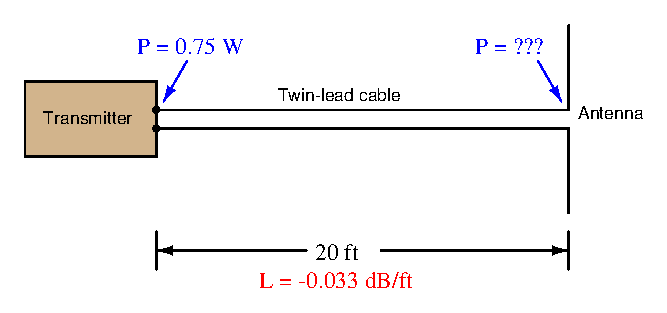
\includegraphics[width=15.5cm]{i01204x01.eps}$$

Kabeltapet på $-0.033$ dB per fot over 20 fot gir et totalt tap på $-0.66$ dB. Dette tilsvarer et effekt{\it forhold} på 0.8590 (dvs. kun 85.90\% av effekten fra senderen når antennen). Dermed blir mottatt antenneeffekt:

$$(0.75 \hbox{ W})(0.8590) = 0.64426 \hbox{ W}$$

Vi kunne nå konvertert 0.64426 watt til dBm og fått det andre svaret (28.091 dBm), men for å illustrere metoden gjør vi hele oppgaven én gang til på en annen måte.

\vskip 10pt

Vi kan angripe oppgaven på nytt ved først å uttrykke senderens utgangseffekt i dBm (0.75 W = 28.751 dBm). Deretter trekker vi bare fra kabeltapet (i dB) for å finne effekten ved antenneinngangen:

$$28.751 \hbox{ dBm} - 0.66 \hbox{ dB} = 28.091 \hbox{ dBm}$$


\vfil \eject

\noindent
{\bf Forberedende quiz:}

Anta at en radiosender leverer 2 watt effekt inn i den ene enden av en tvillingleder-kabel, med antennen koblet i den andre enden. Kabelen er 25 fot lang og har et effekttap på $-0.033$ dB/fot. Beregn effekten mottatt av antennen, i watt.

\begin{itemize}
\item{} 1.175 watt
\vskip 5pt 
\item{} 1.854 watt
\vskip 5pt 
\item{} 24.93 watt
\vskip 5pt 
\item{} 1.654 watt
\vskip 5pt 
\item{} 0.825 watt
\vskip 5pt 
\item{} 1.967 watt
\end{itemize}


\vfil \eject

\noindent
{\bf Forberedende quiz:}

Anta at en radiosender leverer 2.5 watt effekt inn i den ene enden av en koaksialkabel, med antennen koblet i den andre enden. Kabelen er 20 fot lang og har et effekttap på $-0.017$ dB/fot. Beregn effekten mottatt av antennen, i watt.

\begin{itemize}
\item{} 2.312 watt
\vskip 5pt 
\item{} 2.167 watt
\vskip 5pt 
\item{} 1.577 watt
\vskip 5pt 
\item{} 2.404 watt
\vskip 5pt 
\item{} 2.160 watt
\vskip 5pt 
\item{} 2.483 watt
\end{itemize}


%INDEX% Elektronikkrepetisjon: desibel- og effektberegninger

%(END_NOTES)

